\documentclass{standalone}
\usepackage{tikz}
\usetikzlibrary{patterns, positioning}
\usepackage[sfdefault]{ClearSans} %% option 'sfdefault' activates Clear Sans as the default text font
\usepackage[T1]{fontenc}

\begin{document}
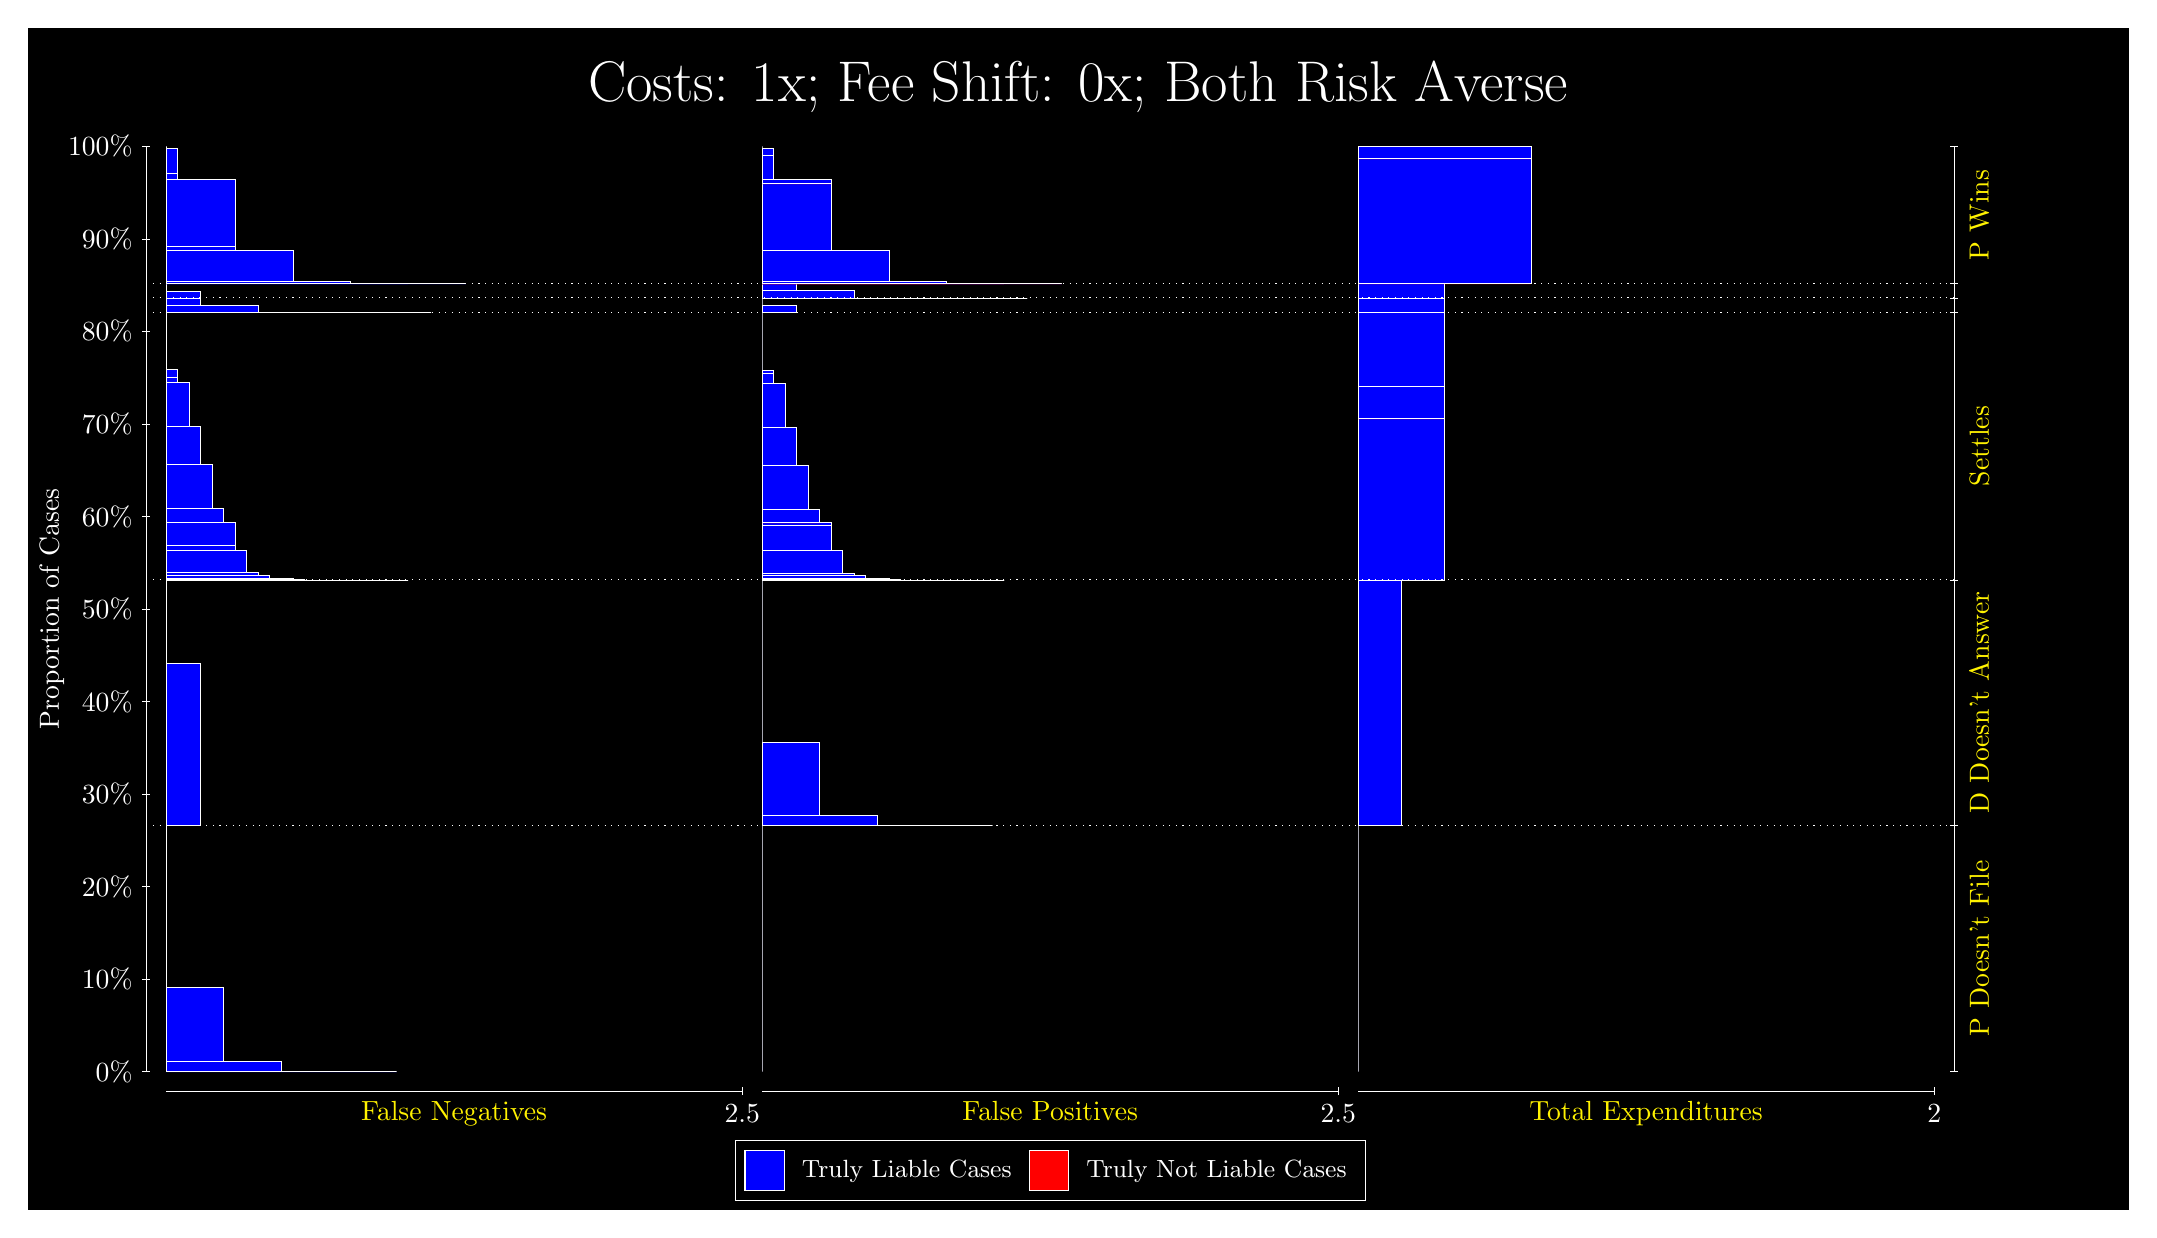
\begin{tikzpicture}
\draw[fill=black] (0,0) rectangle (26.667,15);
\draw[text=white] (0,13.5) rectangle (26.667,15) node[midway] {\huge Costs: 1x; Fee Shift: 0x; Both Risk Averse};
\draw[white, very thin] (1.5,1.75) -- (1.5,13.5);
\node[rotate=90, text=white, anchor=center] at (0.3, 7.625) {Proportion of Cases};
\draw[white, very thin] (1.45,1.75) -- (1.55,1.75);
\node[text=white, anchor=east] at (1.45, 1.75) {0\%};
\draw[white, very thin] (1.45,2.925) -- (1.55,2.925);
\node[text=white, anchor=east] at (1.45, 2.925) {10\%};
\draw[white, very thin] (1.45,4.1) -- (1.55,4.1);
\node[text=white, anchor=east] at (1.45, 4.1) {20\%};
\draw[white, very thin] (1.45,5.275) -- (1.55,5.275);
\node[text=white, anchor=east] at (1.45, 5.275) {30\%};
\draw[white, very thin] (1.45,6.45) -- (1.55,6.45);
\node[text=white, anchor=east] at (1.45, 6.45) {40\%};
\draw[white, very thin] (1.45,7.625) -- (1.55,7.625);
\node[text=white, anchor=east] at (1.45, 7.625) {50\%};
\draw[white, very thin] (1.45,8.8) -- (1.55,8.8);
\node[text=white, anchor=east] at (1.45, 8.8) {60\%};
\draw[white, very thin] (1.45,9.975) -- (1.55,9.975);
\node[text=white, anchor=east] at (1.45, 9.975) {70\%};
\draw[white, very thin] (1.45,11.15) -- (1.55,11.15);
\node[text=white, anchor=east] at (1.45, 11.15) {80\%};
\draw[white, very thin] (1.45,12.325) -- (1.55,12.325);
\node[text=white, anchor=east] at (1.45, 12.325) {90\%};
\draw[white, very thin] (1.45,13.5) -- (1.55,13.5);
\node[text=white, anchor=east] at (1.45, 13.5) {100\%};

\draw[white, very thin] (24.457,1.75) -- (24.457,13.5);
\draw[white, very thin] (24.407,1.75) -- (24.507,1.75);
\node[anchor=west] at (24.407, 1.75) {};
\draw[white, very thin] (24.407,4.8778) -- (24.507,4.8778);
\node[anchor=west] at (24.407, 4.8778) {};
\draw[white, very thin] (24.407,7.9947) -- (24.507,7.9947);
\node[anchor=west] at (24.407, 7.9947) {};
\draw[white, very thin] (24.407,11.394) -- (24.507,11.394);
\node[anchor=west] at (24.407, 11.394) {};
\draw[white, very thin] (24.407,11.575) -- (24.507,11.575);
\node[anchor=west] at (24.407, 11.575) {};
\draw[white, very thin] (24.407,11.755) -- (24.507,11.755);
\node[anchor=west] at (24.407, 11.755) {};
\draw[white, very thin] (24.407,13.5) -- (24.507,13.5);
\node[anchor=west] at (24.407, 13.5) {};

\draw[white, very thin, fill=blue] (1.75,1.75) rectangle (4.6775,1.75);
\draw[white, very thin, fill=blue] (1.75,1.75) rectangle (3.9457,1.7511);
\draw[white, very thin, fill=blue] (1.75,1.7511) rectangle (3.2138,1.8838);
\draw[white, very thin, fill=blue] (1.75,1.8838) rectangle (2.4819,2.8169);
\draw[white, very thin, fill=red] (1.75,2.8169) rectangle (1.75,2.8169);
\draw[white, very thin, fill=blue] (1.75,2.8169) rectangle (1.75,4.8778);
\draw[white, very thin, fill=blue] (1.75,4.8778) rectangle (2.1891,6.939);
\draw[white, very thin, fill=red] (1.75,6.939) rectangle (1.75,6.939);
\draw[white, very thin, fill=blue] (1.75,6.939) rectangle (1.75,7.9947);
\draw[white, very thin, fill=blue] (1.75,7.9947) rectangle (4.8239,7.9947);
\draw[white, very thin, fill=blue] (1.75,7.9947) rectangle (4.2384,7.9947);
\draw[white, very thin, fill=blue] (1.75,7.9947) rectangle (4.092,7.9947);
\draw[white, very thin, fill=blue] (1.75,7.9947) rectangle (3.9457,7.9947);
\draw[white, very thin, fill=blue] (1.75,7.9947) rectangle (3.6529,7.9948);
\draw[white, very thin, fill=blue] (1.75,7.9948) rectangle (3.5065,8.0024);
\draw[white, very thin, fill=blue] (1.75,8.0024) rectangle (3.3602,8.0189);
\draw[white, very thin, fill=blue] (1.75,8.0189) rectangle (3.2138,8.0194);
\draw[white, very thin, fill=blue] (1.75,8.0194) rectangle (3.0674,8.0515);
\draw[white, very thin, fill=blue] (1.75,8.0515) rectangle (2.921,8.0842);
\draw[white, very thin, fill=blue] (1.75,8.0842) rectangle (2.7746,8.3694);
\draw[white, very thin, fill=blue] (1.75,8.3694) rectangle (2.6283,8.4335);
\draw[white, very thin, fill=blue] (1.75,8.4335) rectangle (2.6283,8.7293);
\draw[white, very thin, fill=blue] (1.75,8.7293) rectangle (2.4819,8.8984);
\draw[white, very thin, fill=blue] (1.75,8.8984) rectangle (2.3355,9.4557);
\draw[white, very thin, fill=blue] (1.75,9.4557) rectangle (2.1891,9.9462);
\draw[white, very thin, fill=blue] (1.75,9.9462) rectangle (2.0428,10.5);
\draw[white, very thin, fill=blue] (1.75,10.5) rectangle (1.8964,10.573);
\draw[white, very thin, fill=blue] (1.75,10.573) rectangle (1.8964,10.67);
\draw[white, very thin, fill=blue] (1.75,10.67) rectangle (1.75,10.698);
\draw[white, very thin, fill=red] (1.75,10.698) rectangle (1.75,10.698);
\draw[white, very thin, fill=blue] (1.75,10.698) rectangle (1.75,11.394);
\draw[white, very thin, fill=blue] (1.75,11.394) rectangle (5.1167,11.394);
\draw[white, very thin, fill=blue] (1.75,11.394) rectangle (4.3848,11.394);
\draw[white, very thin, fill=blue] (1.75,11.394) rectangle (3.6529,11.396);
\draw[white, very thin, fill=blue] (1.75,11.396) rectangle (2.921,11.487);
\draw[white, very thin, fill=blue] (1.75,11.487) rectangle (2.1891,11.575);
\draw[white, very thin, fill=red] (1.75,11.575) rectangle (1.75,11.575);
\draw[white, very thin, fill=blue] (1.75,11.575) rectangle (2.1891,11.662);
\draw[white, very thin, fill=red] (1.75,11.662) rectangle (1.75,11.662);
\draw[white, very thin, fill=blue] (1.75,11.662) rectangle (1.75,11.755);
\draw[white, very thin, fill=blue] (1.75,11.755) rectangle (5.5558,11.755);
\draw[white, very thin, fill=blue] (1.75,11.755) rectangle (4.8239,11.755);
\draw[white, very thin, fill=blue] (1.75,11.755) rectangle (4.092,11.785);
\draw[white, very thin, fill=blue] (1.75,11.785) rectangle (3.3602,12.179);
\draw[white, very thin, fill=blue] (1.75,12.179) rectangle (2.6283,12.227);
\draw[white, very thin, fill=blue] (1.75,12.227) rectangle (2.6283,13.076);
\draw[white, very thin, fill=blue] (1.75,13.076) rectangle (1.8964,13.163);
\draw[white, very thin, fill=blue] (1.75,13.163) rectangle (1.8964,13.47);
\draw[white, very thin, fill=red] (1.75,13.47) rectangle (1.75,13.47);
\draw[white, very thin, fill=blue] (1.75,13.47) rectangle (1.75,13.5);
\draw[white, very thin, fill=red] (9.3189,1.75) rectangle (9.3189,1.75);
\draw[white, very thin, fill=blue] (9.3189,1.75) rectangle (9.3189,4.8778);
\draw[white, very thin, fill=red] (9.3189,4.8778) rectangle (12.246,4.8778);
\draw[white, very thin, fill=blue] (9.3189,4.8778) rectangle (12.246,4.8778);
\draw[white, very thin, fill=blue] (9.3189,4.8778) rectangle (11.515,4.8783);
\draw[white, very thin, fill=blue] (9.3189,4.8783) rectangle (10.783,4.9991);
\draw[white, very thin, fill=blue] (9.3189,4.9991) rectangle (10.051,5.9335);
\draw[white, very thin, fill=blue] (9.3189,5.9335) rectangle (9.3189,7.9947);
\draw[white, very thin, fill=red] (9.3189,7.9947) rectangle (12.393,7.9947);
\draw[white, very thin, fill=blue] (9.3189,7.9947) rectangle (12.393,7.9947);
\draw[white, very thin, fill=red] (9.3189,7.9947) rectangle (11.807,7.9947);
\draw[white, very thin, fill=blue] (9.3189,7.9947) rectangle (11.807,7.9947);
\draw[white, very thin, fill=blue] (9.3189,7.9947) rectangle (11.661,7.9947);
\draw[white, very thin, fill=red] (9.3189,7.9947) rectangle (11.515,7.9947);
\draw[white, very thin, fill=blue] (9.3189,7.9947) rectangle (11.515,7.9947);
\draw[white, very thin, fill=red] (9.3189,7.9947) rectangle (11.222,7.9947);
\draw[white, very thin, fill=blue] (9.3189,7.9947) rectangle (11.222,7.9948);
\draw[white, very thin, fill=blue] (9.3189,7.9948) rectangle (11.075,8.0023);
\draw[white, very thin, fill=red] (9.3189,8.0023) rectangle (10.929,8.0023);
\draw[white, very thin, fill=blue] (9.3189,8.0023) rectangle (10.929,8.0184);
\draw[white, very thin, fill=red] (9.3189,8.0184) rectangle (10.929,8.0184);
\draw[white, very thin, fill=blue] (9.3189,8.0184) rectangle (10.929,8.0185);
\draw[white, very thin, fill=blue] (9.3189,8.0185) rectangle (10.783,8.019);
\draw[white, very thin, fill=red] (9.3189,8.019) rectangle (10.636,8.019);
\draw[white, very thin, fill=blue] (9.3189,8.019) rectangle (10.636,8.0508);
\draw[white, very thin, fill=blue] (9.3189,8.0508) rectangle (10.49,8.0806);
\draw[white, very thin, fill=blue] (9.3189,8.0806) rectangle (10.344,8.3653);
\draw[white, very thin, fill=blue] (9.3189,8.3653) rectangle (10.197,8.6915);
\draw[white, very thin, fill=blue] (9.3189,8.6915) rectangle (10.197,8.7193);
\draw[white, very thin, fill=red] (9.3189,8.7193) rectangle (10.051,8.7193);
\draw[white, very thin, fill=blue] (9.3189,8.7193) rectangle (10.051,8.8893);
\draw[white, very thin, fill=blue] (9.3189,8.8893) rectangle (9.9044,9.443);
\draw[white, very thin, fill=blue] (9.3189,9.443) rectangle (9.758,9.9334);
\draw[white, very thin, fill=blue] (9.3189,9.9334) rectangle (9.6116,10.491);
\draw[white, very thin, fill=blue] (9.3189,10.491) rectangle (9.4652,10.622);
\draw[white, very thin, fill=blue] (9.3189,10.622) rectangle (9.4652,10.66);
\draw[white, very thin, fill=blue] (9.3189,10.66) rectangle (9.3189,11.394);
\draw[white, very thin, fill=red] (9.3189,11.394) rectangle (9.758,11.394);
\draw[white, very thin, fill=blue] (9.3189,11.394) rectangle (9.758,11.482);
\draw[white, very thin, fill=blue] (9.3189,11.482) rectangle (9.3189,11.575);
\draw[white, very thin, fill=red] (9.3189,11.575) rectangle (12.686,11.575);
\draw[white, very thin, fill=blue] (9.3189,11.575) rectangle (12.686,11.575);
\draw[white, very thin, fill=blue] (9.3189,11.575) rectangle (11.954,11.575);
\draw[white, very thin, fill=blue] (9.3189,11.575) rectangle (11.222,11.576);
\draw[white, very thin, fill=blue] (9.3189,11.576) rectangle (10.49,11.668);
\draw[white, very thin, fill=blue] (9.3189,11.668) rectangle (9.758,11.755);
\draw[white, very thin, fill=red] (9.3189,11.755) rectangle (13.125,11.755);
\draw[white, very thin, fill=blue] (9.3189,11.755) rectangle (13.125,11.755);
\draw[white, very thin, fill=red] (9.3189,11.755) rectangle (12.393,11.755);
\draw[white, very thin, fill=blue] (9.3189,11.755) rectangle (12.393,11.755);
\draw[white, very thin, fill=red] (9.3189,11.755) rectangle (11.661,11.755);
\draw[white, very thin, fill=blue] (9.3189,11.755) rectangle (11.661,11.785);
\draw[white, very thin, fill=red] (9.3189,11.785) rectangle (10.929,11.785);
\draw[white, very thin, fill=blue] (9.3189,11.785) rectangle (10.929,12.179);
\draw[white, very thin, fill=blue] (9.3189,12.179) rectangle (10.197,13.027);
\draw[white, very thin, fill=red] (9.3189,13.027) rectangle (10.197,13.027);
\draw[white, very thin, fill=blue] (9.3189,13.027) rectangle (10.197,13.076);
\draw[white, very thin, fill=blue] (9.3189,13.076) rectangle (9.4652,13.382);
\draw[white, very thin, fill=blue] (9.3189,13.382) rectangle (9.4652,13.47);
\draw[white, very thin, fill=blue] (9.3189,13.47) rectangle (9.3189,13.5);
\draw[white, very thin, fill=red] (16.888,1.75) rectangle (16.888,1.75);
\draw[white, very thin, fill=blue] (16.888,1.75) rectangle (16.888,4.8778);
\draw[white, very thin, fill=red] (16.888,4.8778) rectangle (17.437,4.8778);
\draw[white, very thin, fill=blue] (16.888,4.8778) rectangle (17.437,7.9947);
\draw[white, very thin, fill=red] (16.888,7.9947) rectangle (17.986,7.9947);
\draw[white, very thin, fill=blue] (16.888,7.9947) rectangle (17.986,10.042);
\draw[white, very thin, fill=red] (16.888,10.042) rectangle (17.986,10.042);
\draw[white, very thin, fill=blue] (16.888,10.042) rectangle (17.986,10.45);
\draw[white, very thin, fill=red] (16.888,10.45) rectangle (17.986,10.45);
\draw[white, very thin, fill=blue] (16.888,10.45) rectangle (17.986,11.394);
\draw[white, very thin, fill=red] (16.888,11.394) rectangle (17.986,11.394);
\draw[white, very thin, fill=blue] (16.888,11.394) rectangle (17.986,11.575);
\draw[white, very thin, fill=red] (16.888,11.575) rectangle (17.986,11.575);
\draw[white, very thin, fill=blue] (16.888,11.575) rectangle (17.986,11.755);
\draw[white, very thin, fill=red] (16.888,11.755) rectangle (19.083,11.755);
\draw[white, very thin, fill=blue] (16.888,11.755) rectangle (19.083,13.344);
\draw[white, very thin, fill=red] (16.888,13.344) rectangle (19.083,13.344);
\draw[white, very thin, fill=blue] (16.888,13.344) rectangle (19.083,13.5);
\draw[white, dotted] (1.5,4.8778) -- (24.457,4.8778);
\draw[white, dotted] (1.5,7.9947) -- (24.457,7.9947);
\draw[white, dotted] (1.5,11.394) -- (24.457,11.394);
\draw[white, dotted] (1.5,11.575) -- (24.457,11.575);
\draw[white, dotted] (1.5,11.755) -- (24.457,11.755);
\draw[white, very thin] (1.75,1.5) -- (9.0689,1.5);
\node[text=yellow, anchor=north] at (5.4094, 1.5) {False Negatives};
\draw[white, very thin] (9.0689,1.45) -- (9.0689,1.55);
\node[text=white, anchor=north] at (9.0689, 1.45) {2.5};

\draw[white, very thin] (9.3189,1.5) -- (16.638,1.5);
\node[text=yellow, anchor=north] at (12.978, 1.5) {False Positives};
\draw[white, very thin] (16.638,1.45) -- (16.638,1.55);
\node[text=white, anchor=north] at (16.638, 1.45) {2.5};

\draw[white, very thin] (16.888,1.5) -- (24.207,1.5);
\node[text=yellow, anchor=north] at (20.547, 1.5) {Total Expenditures};
\draw[white, very thin] (24.207,1.45) -- (24.207,1.55);
\node[text=white, anchor=north] at (24.207, 1.45) {2};

\node[text=yellow, centered, rotate=90] at (24.777, 3.3139) {P Doesn't File};
\node[text=yellow, centered, rotate=90] at (24.777, 6.4362) {D Doesn't Answer};
\node[text=yellow, centered, rotate=90] at (24.777, 9.6946) {Settles};


\node[text=yellow, centered, rotate=90] at (24.777, 12.627) {P Wins};

\draw (12.978300999999998,1.5) node[draw=none] (baseCoordinate) {};
\begin{scope}[align=center]
        \matrix[scale=0.5, draw=white, below=0.5cm of baseCoordinate, nodes={draw}, column sep=0.1cm]{
            \node[rectangle, draw, minimum width=0.5cm, minimum height=0.5cm, fill=blue] {}; &
            \node[draw=none, font=\small, text=white] (B) {Truly Liable Cases}; &
            \node[rectangle, draw, minimum width=0.5cm, minimum height=0.5cm, fill=red] {}; &
            \node[draw=none, font=\small, text=white] (B) {Truly Not Liable Cases}; \\
            };
\end{scope}

\end{tikzpicture}
\end{document}